\section{Introduction}
\label{sec:intro}

Major industrial players are increasingly embracing resource disaggregation,
where memory and storage are physically separated from computation. This
segregation provides numerous opportunities for increased scalability, power
efficiency, and cost savings, but also raises fundamental performance
bottlenecks~\cite{requirements}. Disaggregating primary storage (i.e,
byte-addressable main memory) remains an unsolved challenge given the
dramatic (e.g., $20\times$) increase in access latency when moving from
on-die cache ($\approx 50$ ns) to network-attached options (often on the
order of 1 us). As a result, many previous systems use application
transparent remote memory only as a form of backing store for infrequently
accessed data~\cite{job_throughput,infiniswap,leap,legoos}.

%% %%State of the world
%% Disaggregated computing promises higher resource density, increased
%% power-efficiency, and flexible application scalability in datacenters.
%% While enticing, these benefits have remained mostly untapped due to
%% the proportionally large overhead of accessing remote resources.
%% Nowhere is this disparity more noticeable than remote memory.
%% Separating CPUs last level cache from their main memory incurs at
%% least a 20x overhead (approximately 50\textit{ns} to 1\textit{us}).
%% The cost is only acceptable for select asynchronous workloads, such as
%% paging out infrequently touched data~\cite{infiniswap,legoos,leap},
%% but are entirely unrealistic when multiple CPUs require consistency
%% for frequent reads and writes to shared remote memory.

Alternatively, others have designed high-performance, special-purpose
distributed data structures run over
RDMA~\cite{farm,erpc,herd,fasst,pilaf,cell,sonuma,storm}. These
non-transparent systems trade generality for performance; handling millions
of operations per second. They all require a CPU be co-resident with remote
memory to act as a RDMA coordinator. This design paradigm of CPU/remote
memory collocation is at odds with the goals of disaggregation; demanding new
approaches for remote resource coordination. Researchers have considered a
variety of trade-offs along this spectrum~\cite{aguilera2019designing,
disandapp, amanda-hotnets,beyond,requirements}. Ideally, systems could
leverage what is sometimes called passive remote~\cite{clover} or
far~\cite{aguilera2019designing} memory, which does not have local
computation attached. Rather, all accesses are remote, using hardware
primitives like one-sided RDMA.

Relatively few systems have been proposed to leverage passive remote
memory, and those that have~\cite{reigons,clover} are designed to
support read-heavy workloads on any shared resources.  Their reason
for avoiding writes is fundamental: ensuring consistency in the face
of concurrent writes is expensive. Lock acquisition and revocation
requires multiple round trips which would devastate throughput.
Conversely, optimistic schemes break down in the face of contention
and typically fall back to even more expensive recovery operations.

One recent system, Clover~\cite{clover}, attempts to decrease the cost
of conflicts by separating (potentially contented) metadata operations
from the memory updates themselves.  While effective for read-mostly
workloads, Clover simply delays the inevitable, and metadata
contention quickly becomes the bottleneck at even modest update rates.
Indeed, published results show that Clover's throughput drops by more
than a factor of four when moving from a read-only to 50\%-write
workload~\cite[Fig. 7]{clover}.
%
%Even with an intelligent concurrent algorithm to opportunistically
%avoid lock acquisition the problem is pervasive due to the natural
%concurrency and relatively high latency of remote memory.
%%
%In the opportunistic case write conflicts due to inconsistencies in
%local caches occur frequently when resources are contested.
%% Figure~\ref{fig:conflicts} shows the number of conflicting concurrent 
%% writes to shared resources as the number of clients requesting the
%% resources are increased.
%
%% \begin{figure}
%%     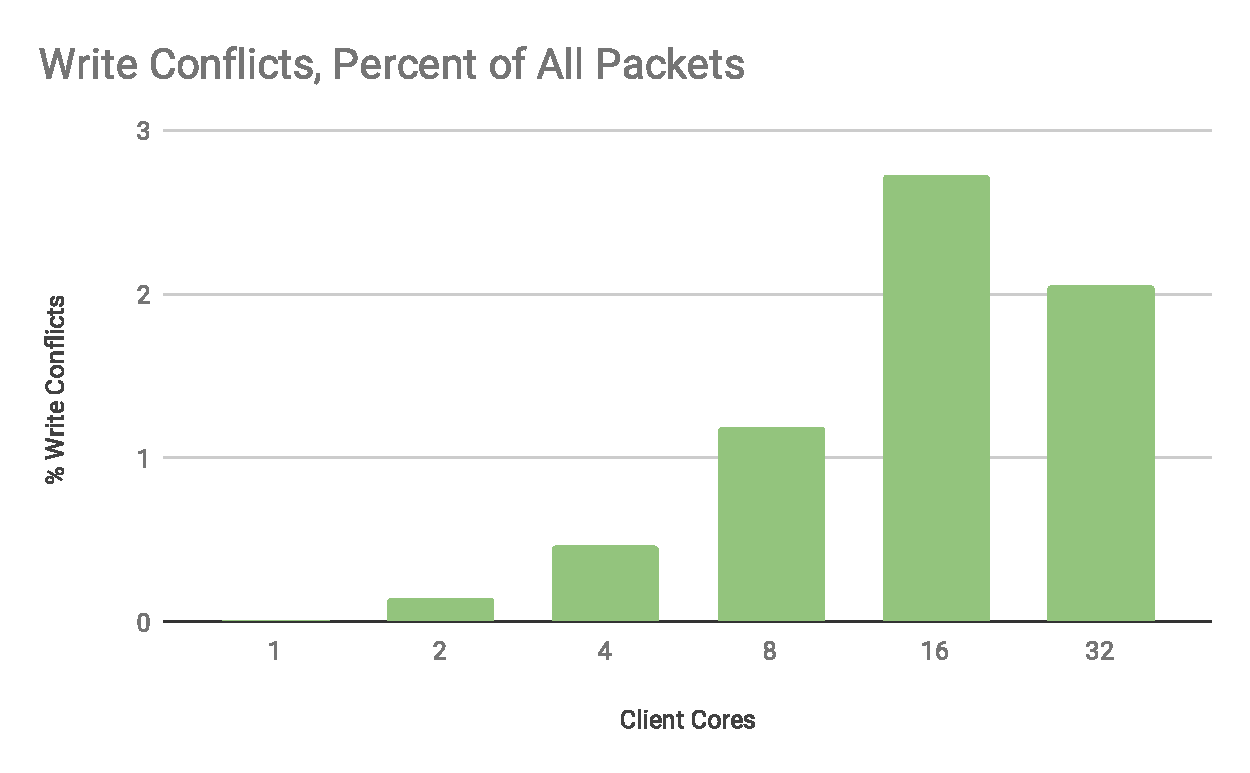
\includegraphics[width=0.45\textwidth]{fig/write_conflicts.pdf}
%%     \caption{Clover write conflicts grow with the number of clients
%%     (50\% write zipf 0.99 distribution)\todo{redo with 64 cores and
%%     writes only}}
%%     \label{fig:conflicts}
%% \end{figure}
%
%% In clovers specific case its throughput is severely degraded under
%% write heavy workloads. Figure~\ref{fig:clover_tput} shows clovers
%% reported throughput drop when subjected to a 50\% write workload.
%
%% \begin{figure}
%%     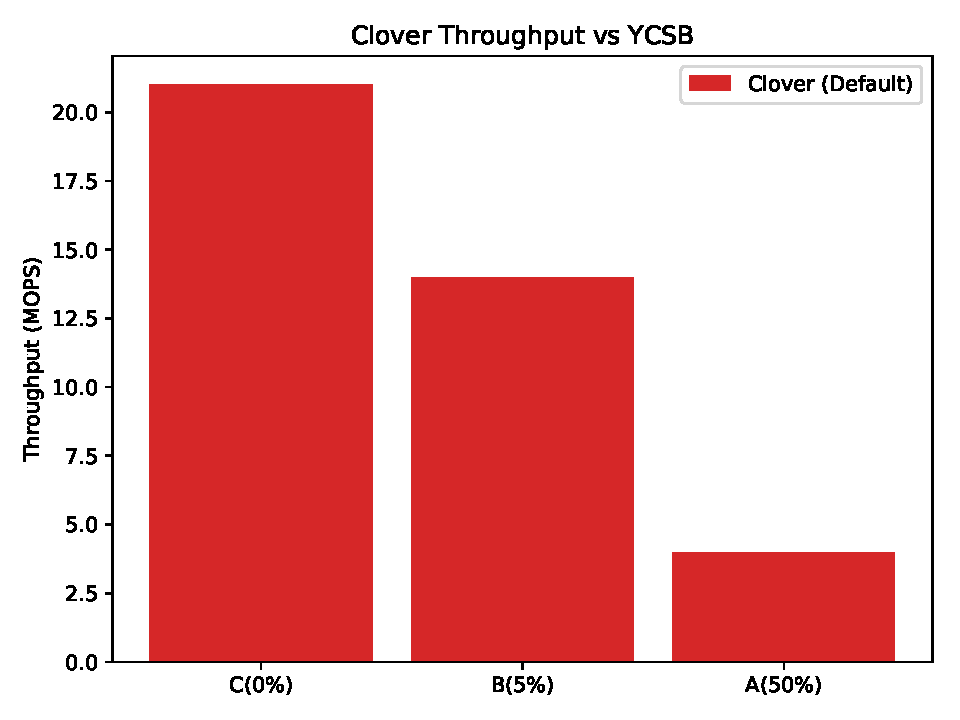
\includegraphics[width=0.45\textwidth]{fig/clover_tput.pdf}
%%     \caption{Clover throughput degradation as a function of write
%%     workload\todo{redo on my setup for consistent ops/s}}
%%     \label{fig:clover_tput}
%% \end{figure}
%
The key issue with designs like Clover is the requirement that
individual clients resolve any conflicts themselves, resulting in
extremely expensive operations in the worst case.  The authors report
that Clover requires five round trips to remote memory in the
99th-percentile case with just a 5\%-write workload~\cite[Table 2]{clover}.

The obvious alternative to completely distributed contention
resolution is to have a central coordinator that manages remote memory
accesses.  Prior work has suggested the potential benefits of a
distributed memory controller~\cite{disandapp}, but to our knowledge
none have yet been built or proposed with existing hardware.  The
authors of Clover evaluate using a commodity server in such a role
(which they refer to as pDPM-central) and discard it as a scalability
bottleneck that also increases the number of network hops between a
node and its remote memory~\cite{clover}.  While an end host is indeed
ill-suited for this purpose, an in-network device, on
the other hand, could be an ideal location to provide such a service:
it is, after all, on-path, and, if suitably located, may be in a
position to observe---and even avoid---conflicting access
requests before they reach remote memory.

In this paper we explore the potential for a programmable top-of-rack
(TOR) switch to mediate remote memory accesses.  We observe that if
all remote reads and writes are performed within a single rack---which
is often the case in existing RDMA deployments---the TOR is in a unique
position to observe---and serialize---remote memory operations.
%% This fact allows it to act as a centralized serialization point,
%% where the last instance of read/write concurrency are the memory
%% attached egress ports of the switch.
%Figure~\ref{fig:overview} illustrates the
%organization of a disaggregated rack, and highlights different
%proposed points of coordination for reads and writes.
Moreover, if the TOR is able to parse and modify requests in flight, it
can even resolve conflicts before they reach the remote memory,
effectively recovering from optimistic write failures ``for free.''
Finally, if clients retain the ability to resolve conflicts
themselves (albeit at a significant cost to performance) the TOR can
serve simply as a form of soft-state performance-enhancing proxy;
conflicts that it fails to avoid will result in
decreased performance as opposed to incorrect semantics.

As a proof of concept we design a prototype software-based TOR that
interposes on the Clover protocol and resolves write conflicts in
flight. Our conflict-detection algorithm uses knowledge of Clover's
metadata structures to detect write conflicts using a small amount of
cached state (only a few bytes per key/value pair). Conflict
resolution is performed directly on the in-flight RDMA packets by
steering their destination virtual addresses to the most up-to-date
read and write locations in Clover's key/value store. This technique
is complete and safe: it resolves all read and write conflicts for
keys that it caches, and reverts to native Clover performance for
those it does not. As in-network SRAM is expensive we show that our
technique can trade completeness for memory savings while still
achieving performance gains. Our preliminary evaluation with a 50/50
read/write workload shows throughput gains of $1.42\times$ when
caching all keys, and gains of $1.34\times$ when using only 128 bytes
of in-network memory to correct conflicts for the 8 most-popular keys
in a Zipf request distribution.
